\documentclass[12pt]{article}
\usepackage{amsmath}
\usepackage{graphicx}
\usepackage{wrapfig}
\usepackage{booktabs}
\usepackage[letterpaper, margin=1in]{geometry}
\usepackage{fancyhdr}
\pagestyle{fancy}
\fancyhead[R]{Inductors and Capacitors}
\fancyfoot[C]{\thepage}
\renewcommand{\headrulewidth}{1pt}
\renewcommand{\footrulewidth}{1pt}
\renewcommand{\baselinestretch}{1.0}
\newcommand{\twoobjects}[2]{%
  \leavevmode\vbox{\hbox{#1}\nointerlineskip\hbox{#2}}%
}
\title{Inductors and Capacitors}
\date{}
\begin{document}
    \section*{Problem 6.5}
    \par The current in a 20 $mH$ inductor is known to be
    \[
    i(t) =
        \begin{cases}
            40\ mA & t \le 0 \\
            A_1 e^{-10000t} + A_2 e^{-40000t}\ A & t \ge 0
        \end{cases}
    \]
    \textit{i)} Choose the correct expression for the voltage across the inductor
    for $t > 0$:
    \[
        v(t) = L \frac{di}{dt}
    \]
    \[
        v(t) = (20*10^{-3}) * \frac{d}{dt} (A_1 e^{-10000t} + A_2 e^{-40000t})
    \]
    \[
        v(t) = (20*10^{-3}) * (-10000A_1e^{-10000t}-40000A_2e^{-40000t})
    \]
    \[
        v(t) = 200A_1e^{-10000t}-800A_2e^{-40000t}
    \]
    This is the voltage across the inductor at time $t > 0$. The initial
    voltage in the inductor is, $v(0) = 28$ V. Since $v(t) = 200A_1e^{-10000t}-800A_2e^{-40000t}
    $, $v(0) = 200A_1 - 800A_2$.
    \begin{equation}
        28 = 200A_1 - 800A_2
    \end{equation}
    The equation for the current can then be used, $i(t) = A_1 e^{-10000t} +
    A_2 e^{-40000t}$, where \\ $i(0) = A_1 + A_2$
    \begin{equation}
        40 * 10^{-3} = A_1 + A_2
    \end{equation}
    Solving these two equations:
    \[
    A_1 = 0.1
    \]
    \[
    A_2 = -0.06
    \]
    Now to get the final answer for the voltage as a function of time, the
    values of $ A_1$ and $ A_2$ are substituted:
    \[
        \boxed{v(t) = -20 e^{-10000t} + 48 e^{-40000t}}
    \]
    \textit{ii)} Find the time, greater than zero, when the power at the terminals
    of the inductor is zero.
    \[
        power = iv = iL \frac{di}{dt}
    \]
    \[
        power = (0.1e^{-10000t} - 0.06e^{-40000t})(-20e^{-10000t} + 48e^{-40000t})
    \]
    \[
        power = -2e^{-20000t} + 4.8e^{-50000t} + 1.2e^{-50000t} - 2.88e^{-80000t}
    \]
    \[
        power = -2e^{-20000t} + 6e^{-50000t} - 2.88e^{-80000t}
    \]
    \[
        0 = -2e^{-20000t} + 6e^{-50000t} - 2.88e^{-80000t}
    \]
    Setting $e^{-20000t} = x$,
    \[
        0 = -2x + 6x^{2.5} + 2.88x^{4}
    \]
    \[
        x = 0 \quad
        x = (\frac{5}{12})^{\frac{1}{1.5}}
    \]
    \[
        e^{-20000t} = (\frac{5}{12})^{\frac{1}{1.5}}
    \]
    \[
        \boxed{t = 29.18\ \mu s}
    \]
    \section*{Problem 6.12}
    Initially there was no energy stored in the 5 H inductor in the circuit in
    the following figure when it was placed across the terminals of the voltmeter.
    At t = 0 the inductor was switched instantaneously to position b where it
    remained for 1.6 s before returning instantaneously to position a. The
    d'Arsonval voltmeter has a full-scale reading of 28 V and a sensitivity of
    $1000\ \Omega / V$. \\
    \textit{i)} What will the reading of the voltmeter be at the instant the switch
    returns to position a if the inertia of the d'Arsonval movement is negligible?
    \[
        i(t) = \frac{1}{L} \int_0^t v(t)\ dt
    \]
    \[
        i(t) = \frac{1}{5} \int_0^t (3*10^{-3})\ dt
    \]
    \[
        i(t) = \frac{3*10^{-3}}{5}t
    \]
    \[
        i(1.6) = \frac{3*10^{-3}}{5}(1.6) = 0.00096\ A
    \]
    The full scale reading of the meter is 28 V, and the sensitivity is $1000\
    \Omega / V$, therefore, the resistance of the meter is  $28 * 1000\ \Omega
    \frac{V}{V}$ = $28000\ \Omega$.
    \[
        V = iR
    \]
    \[
        V = (0.00096)(28000) = \boxed{26.88\ V}
    \]
    \section*{Problem 6.14}
    The voltage at the terminals of the capacitor in is known to be:
    \[
        v(t) =
        \begin{cases}
            -10\ V & t \le 0 \\
            40 - 1e^{-1000t}(50\cos(500t) + 20\sin(500t))\ V & t \ge 0
        \end{cases}
    \]
    where $t$ is in seconds. Assume $C = 0.8\ \mu F$. \\
    \textit{i)} Find the current in the capacitor for $t > 0$.
    \[
        i(t) = C \frac{dv}{dt}
    \]
    \[
        i(t) = (0.8) \frac{d}{dt}(40 - 1e^{-1000t}(50\cos(500t) + 20\sin(500t)))
    \]
    \[
        i(t) = 0.8e^{-1000t}(45000\sin(500t) + 40000\cos(500t))
    \]
    \[
        i(t) = e^{-1000t}(36000\sin(500t) + 32000\cos(500t))\ A
    \]
    \[
        \boxed{i(t) = e^{-1000t}(36\sin(500t) + 32\cos(500t))\ mA}
    \]
    \textit{ii)} How much energy (in millijoules) is stored in the capacitor at
    $t=\infty$?
    \[
        v(t) = 40, t = \infty
    \]
    \[
        w = \frac{1}{2} C v^2
    \]
    \[
        w = \frac{1}{2} (0.8) (40)^2
    \]
    \[
        \boxed{w = 0.64\ mJ}
    \]
    \section*{Problem 6.34}
    \begin{figure}[h]
        \centering
        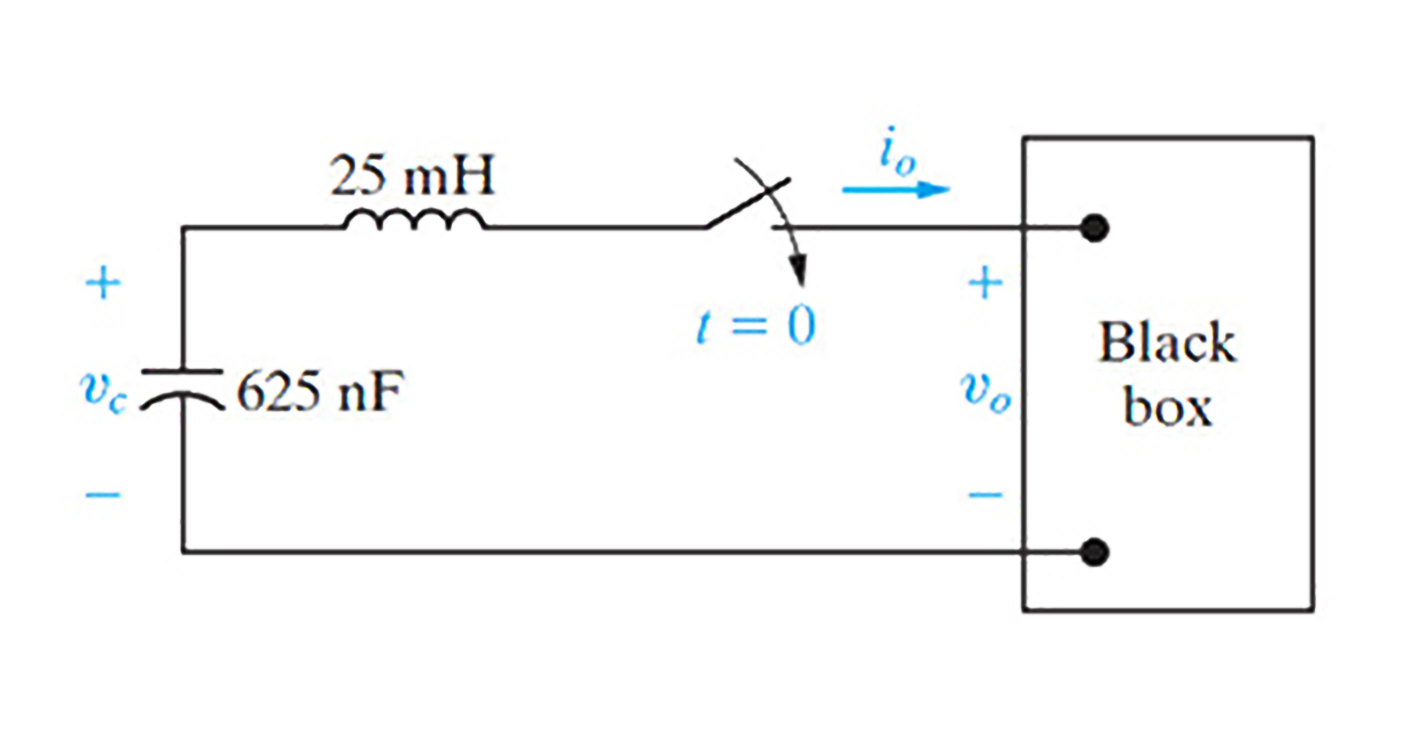
\includegraphics[width=0.6\textwidth]{Figure 1.png}
    \end{figure}
    At $t=0$ a series-connected capacitor and inductor are placed across the
    terminals of a black box, as shown in Figure 1. For $t>0$:
    \[
        i_0 = 1.5e^{-16000t} - 0.5e^{-4000t}\ A
    \]
    \noindent Voltage across the capacitor: $v(0) = -50\ V$
    \[
        v(t) = -\frac{1}{C} \int_0^t i_0 dt + v(0)
    \]
    \[
        v(t) = -\frac{1}{625*10^{-9}} \int_0^t (1.5e^{-16000t} - 0.5e^{-4000t}) dt -
        50
    \]
    \[
        v(t) = -\frac{1}{625*10^{-9}} * \frac{1}{32000}
        (e^{-16000t}(4e^{12000t}-3)-1) - 50
    \]
    \[
        v(t) = -50(e^{-16000t}(4e^{12000t} - 3) -1) - 50
    \]
    \[
        v(t) = -50e^{-16000t}(4e^{12000t} - 3)
    \]
    \[
        v(t) = 150e^{-16000t} - 200e^{-4000t}\ V
    \]
    Voltage across the inductor:
    \[
        v(t) = L \frac{di}{dt}
    \]
    \[
        v(t) = 25*10^{-3} \frac{d}{dt}(1.5e^{-16000t} - 0.5e^{-4000t})
    \]
    \[
        v(t) = e^{-16000t}(50e^{12000t} - 600)
    \]
    $v_0$ will equal $v_c - v_l$:
    \[
        v_0 = (150e^{-16000t} - 200e^{-4000t}) - (e^{-16000t}(50e^{12000t} - 600))
    \]
    \[
        \boxed{v_0 = 750e^{-16000t} - 250e^{-4000t}\ V}
    \]
\end{document}
